\documentclass[tikz,border=5pt]{standalone}
\usepackage{tikz}
\usepackage{amsmath}
\usetikzlibrary{arrows.meta,patterns}
\definecolor{nebula}{HTML}{6366F1}
\definecolor{spark}{HTML}{14B8A6}
\definecolor{ink}{HTML}{334155}
\begin{document}
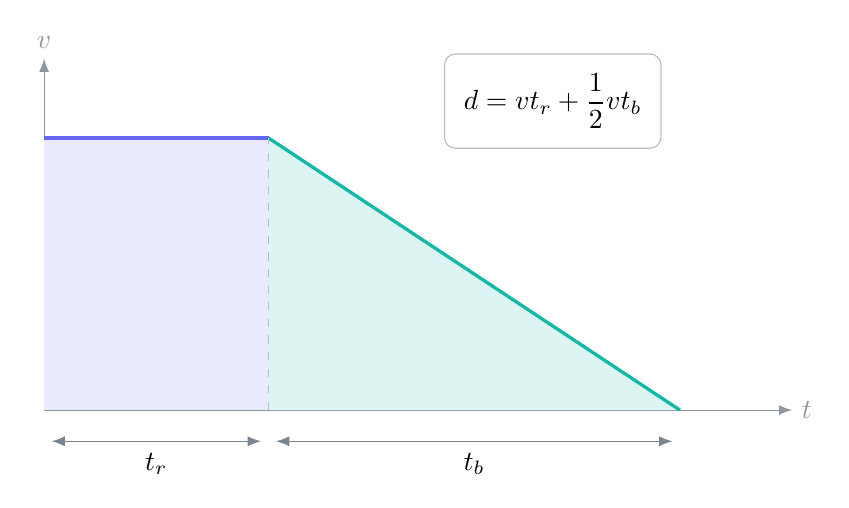
\begin{tikzpicture}[font=\sffamily,>=Latex,x=.95cm,y=.72cm]
  \draw[->,ink!55] (0,0)--(10,0) node[right] {$t$};
  \draw[->,ink!55] (0,0)--(0,6.2) node[above] {$v$};
  \fill[nebula!14] (0,0) rectangle (3,4.8);
  \fill[spark!15] (3,0)--(3,4.8)--(8.5,0)--cycle;
  \draw[very thick,nebula] (0,4.8)--(3,4.8);
  \draw[very thick,spark] (3,4.8)--(8.5,0);
  \draw[dashed,ink!35] (3,0)--(3,4.8);
  \draw[<->,ink!65] (.1,-.55)--(2.9,-.55);
  \node[fill=white,inner sep=2pt] at (1.5,-.95) {$t_r$};
  \draw[<->,ink!65] (3.1,-.55)--(8.4,-.55);
  \node[fill=white,inner sep=2pt] at (5.75,-.95) {$t_b$};
  \node[draw=ink!35,rounded corners=4pt,fill=white,inner sep=7pt] at (6.8,5.45)
    {$d=v t_r+\dfrac12v t_b$};
\end{tikzpicture}
\end{document}
